\section{Evaluation}
We analyze over 3,000,000 SCOPE jobs over a period of several days that run on five data centers at Microsoft. 
In summary, our experiments illustrate the following:

\begin{itemize}
\item \emph{What is the proportion of time spent in native vs. non-native job vertices?}
Between \nonNativeTimeL{} and \nonNativeTimeU \% of data center time is spent in job vertices that run managed code.

\item \emph{What proportion of time can be optimized having the current list of methods with C++ implementation?} 
With the current list of intrinsicable methods we can optimize up to \optimizableU{} \% of data center time.

\item \emph{What proportion of time can be optimized by extending the list of methods with C++ implementation? 
Which methods should be the most important for C++ implementation?}
By increasing the list of intrinsics and optimizing all inlineable methods we can optimize up to \potentiallyOptimizableU{} \% of data center time. 
Furthermore, we conclude that \emph{String} methods are the most important .NET framework methods amenable for C++ implementations.


\end{itemize}

\subsection{Experimental Setup}
To understand performance bottlenecks in SCOPE jobs we analyze over 3,000,000 jobs across 5 data centers.
Table~\ref{tb:projects} lists, for each data center, the number of analyzed jobs along with their CPU time measured in hours.
We observe that number of jobs and CPU time significantly vary between data centers. 
For example, data center \emph{cosmos15} run the highest proportion of jobs we analyze, while \emph{cosmos9} run the most expensive jobs. 
This is expected because different data centers are usually tailored for different types of jobs. 

\begin{table}[ht]
\centering
\begin{tabular}{lrr}

  Data center & Number of jobs & CPU time (in hours) \\
 \midrule
cosmos8 & 375,974 & 28,559,063 \\
cosmos9 & 171,203 & 40,714,052 \\
cosmos11 & 851,222 & 23,312,271\\
cosmos14 & 474,911 & 21,299,039\\
cosmos15 & 1,200,026 & 31,324,407 \\
\midrule
Total: & 3,073,336 & 145,208,834\\
\midrule

\end{tabular}
 
 \caption{Analyzed jobs and their CPU time
 \label{tb:projects}}
\end{table}




\subsection{Native vs. Non-Native Time}
Before optimizing non-relational logic in SCOPE jobs, it is important to understand how much time is spent in job vertices that run non-relational code. 
The analysis of C++ code returns for every job vertex whether it runs as native or managed code. 
Combined with data from \emph{Runtime Statistics} we also find how much time is taken by every job vertex.

Figure~\ref{fig:nativeVsNonNative} illustrates our results.
It shows for every data center how much time is spent in native and non-native vertices. 
Grey area denotes few exceptional vertices for which the analysis can not certainly distinguish the code that runs inside a vertex. 
For example, sometimes the analysis does not detect any source of managed code in a vertex that supposedly runs C\# code. 
The time of such vertices we assign to gray area.

We conclude from Figure~\ref{fig:nativeVsNonNative} that time spent in non-native code represents a large fraction of data center time.
For example, in cosmos9, the time spent in native vertices contributes to only 21.30\% of data center time. 
These results illustrate the potential of optimizing the non-relational code and it influence on data center time.

\begin{figure*}[ht]
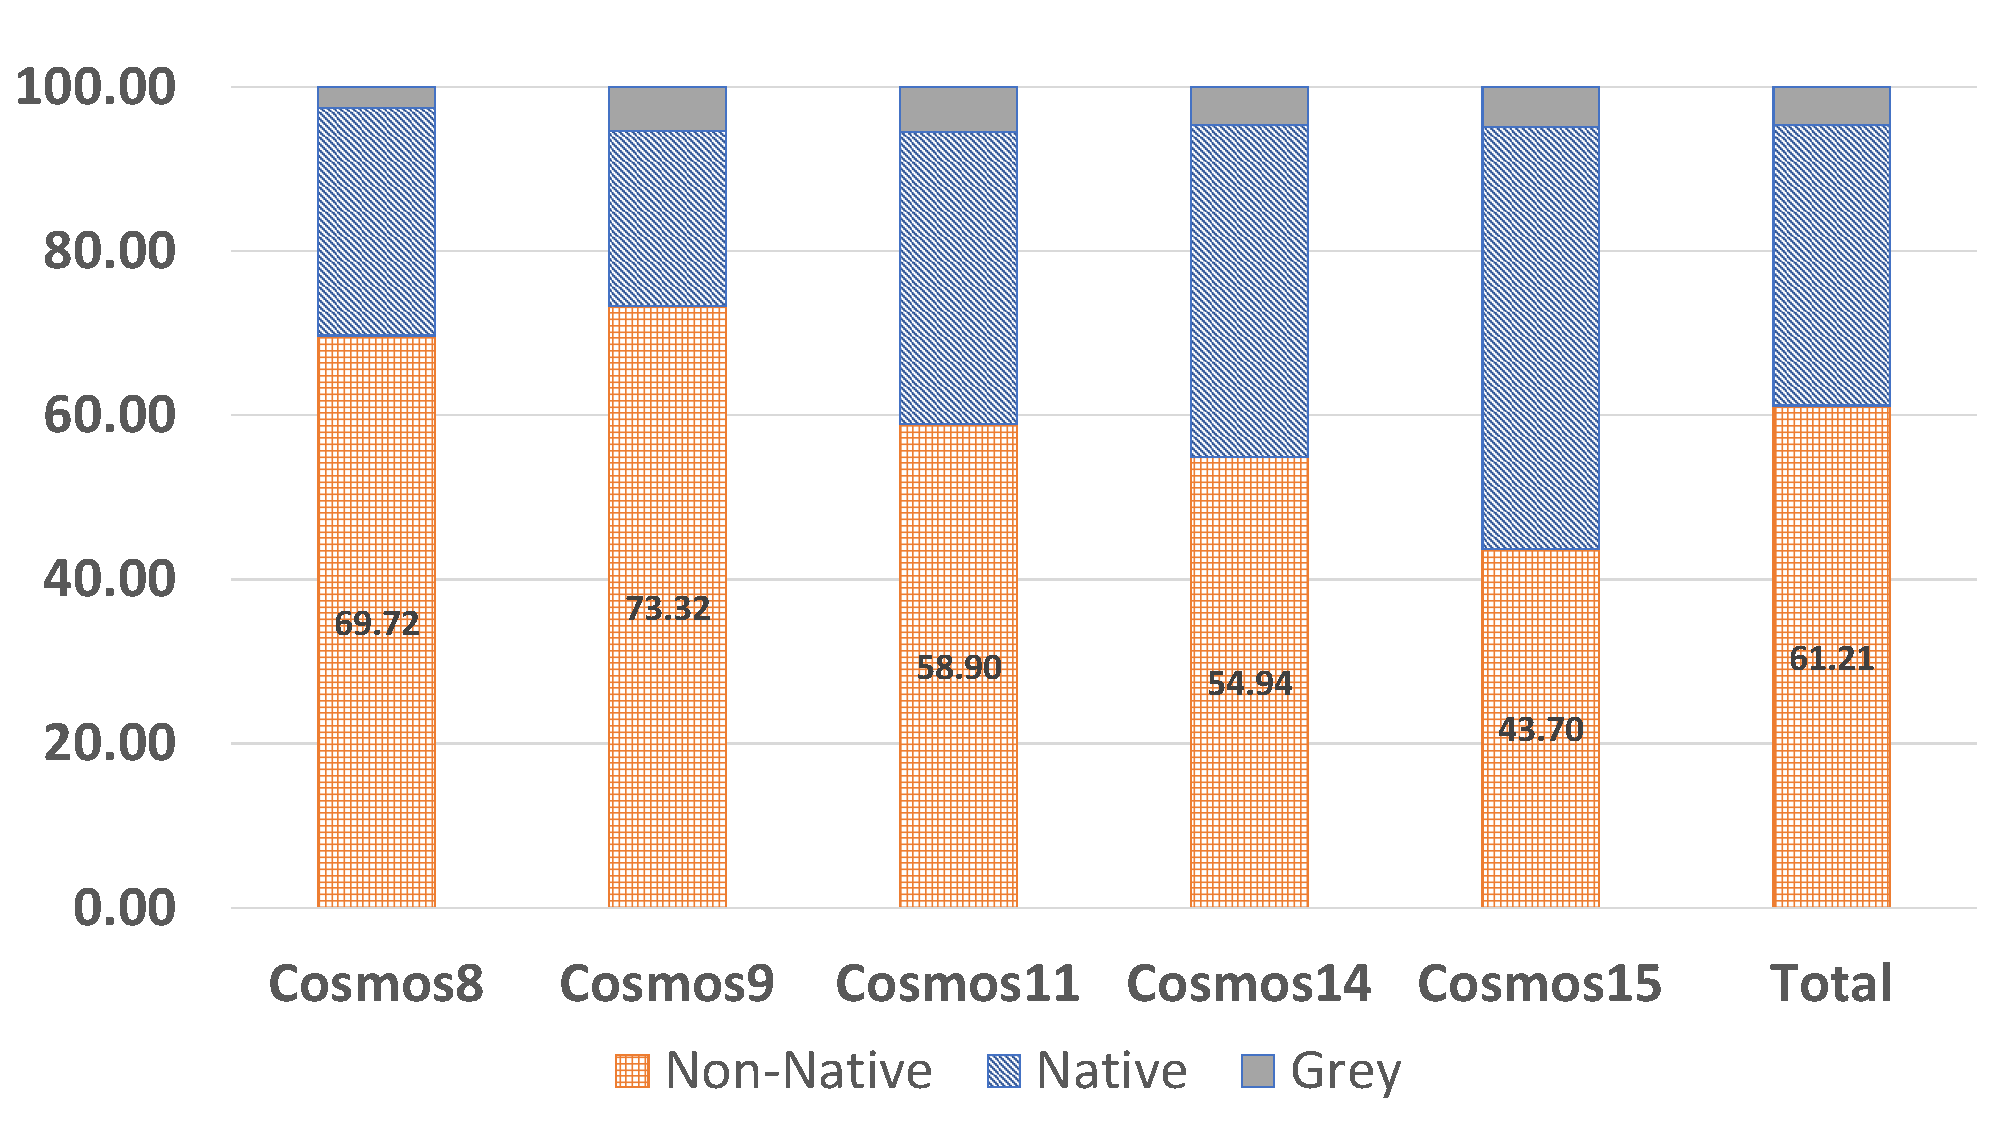
\includegraphics[width=2\columnwidth]{graphs/proportions.pdf}
\caption{Time spent in native vs. non-native vertices}
\label{fig:nativeVsNonNative}
\end{figure*}

\subsection{Optimizable Job Vertices}


We say a job vertex is \emph{optimizable} if it has as the only source of managed code inlineable methods that have only calls to existing intrinsics. 
Optimizable vertices are important because we can quantify how much data center time we can optimize considering the current list of intrinsics. 
Moreover, by inlining method calls, we expect an entire vertex to run as native code, which should significantly improve the vertex execution time.

Figure~\ref{fig:optimizable} shows the proportion of CPU time of \emph{optimizable} vertices relative to data center time and to time spent in vertices with non-native code. 
We observe that with the current list of intrinsics we can optimize a relatively small proportion of data center time. 
For example, in cosmos9 that runs the most expensive jobs, we can optimize at most 0.01\% of data center time. 
The situation is slightly better in cosmos14 and cosmos15, but in these data centers, the proportion of non-native time is relatively lower compared to cosmos9.

The crucial observation is that given results illustrate only the time in data centers that can be affected by inlining method calls in optimizable vertices. 
To measure the actual performance improvement it is necessary to rerun every optimized job. 
Further details on performance improvements for several jobs we optimize are given in Section~\ref{sec:caseStudy}.

\begin{figure}[ht]
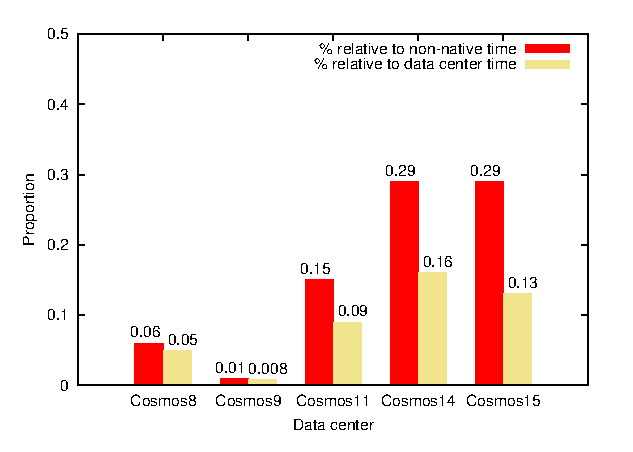
\includegraphics[scale=0.8]{graphs/optimizable}
\caption{Optimizable job vertices}
\label{fig:optimizable}
\end{figure}

\subsection{Potential for C++ Translation}
To motivate the importance of providing the C++ implementation for more framework methods, we measure how much time is spent in the following type of vertices:
\begin{itemize}
\item Vertices with .NET framework calls as the only source of managed code
\item Vertices with .NET framework calls or calls to inlineable methods as the only source of managed code
\end{itemize}
We call these vertices \emph{potentially optimizable}, because they can run as native by increasing the list of intrinsics.

Figure~\ref{fig:potentially} shows the proportion of time spent in potentially optimizable vertices relative to data center time. 
We measure the proportions by assuming that all .NET framework methods have C++ implementation.
Results illustrate that we can optimize between \potentiallyOptimizableL{} and \potentiallyOptimizableU{} \% of data center time by just increasing the list of intrinsics. 
Even though \potentiallyOptimizableL{} \% of time spent in cosmos9 looks relatively low, it counts for almost 407,140 CPU hours for a period of several days. 
Knowing this type of impact motivates the future work on enabling more C++ translation of framework methods.

\begin{figure}[ht]
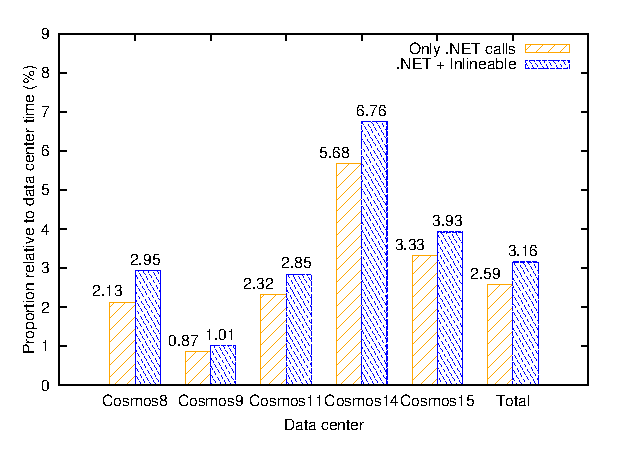
\includegraphics[scale=0.8]{graphs/potentiallyOptimizable}

\caption{Potentially optimizable job vertices}
\label{fig:potentially}
\end{figure}

\subsubsection{Most Relevant .NET Framework Methods}
Assuming that all .NET framework methods have C++ implementation is unrealistic. 
To provide more insights on the framework methods that actually matter, we perform two types of study:
the study of the most relevant methods considering the execution time of a vertex and the study of the most important method types. 

For the first study, we take all .NET framework methods called in potentially optimizable vertices and rank them based on the vertex execution time. 
Table~\ref{tb:rankedMethods} shows for every data center ten most important framework methods. 
The last row further illustrates how much data center time can be optimized if all methods in the list become intrinsics.
We further highlight methods that appear to be relevant across many data centers.
For example, \emph{System.String.ToLower} and \emph{System.String.Concat} are among the most relevant methods across all data centers.
Furthermore, if the native implementation is provided for the first ten methods in cosmos14, the data center it would be enough to optimize more than 5\% of data center time.

\begin{table*}[ht]
\small
 \begin{tabular}{@{}llllp{3.5cm}@{}}

  Cosmos8 & Cosmos9 & Cosmos11 & Cosmos14 & Cosmos15 \\
 \midrule
Convert.ToInt64 & \textbf{String.Equals} & String.Replace & \textbf{DateTime.ToString} & \textbf{String.ToLower} \\
Int32.Parse & \textbf{String.ToLower} & \textbf{String.ToLower} & String.IndexOf & String.LastIndexOf \\
\textbf{String.ToLower} & Int32.Parse & String.ToUpper & DateTime.ToLocalTime & \textbf{DateTime.ToString}\\
\textbf{String.Concat} & String.Replace & \textbf{String.Concat} & \textbf{String.ToLower} & \textbf{String.Concat}\\
String.Replace & Convert.ToDateTime & String.Trim & String.ToUpper & Convert.ToUInt64 \\
Double.Parse & Regex.isMatch & Math.Max & Regex.IsMatch & Enumerable.SelectMany \\
Math.Round& DateTime.ToUniversalTime & \textbf{String.Equals} & \textbf{String.Equals} & Enumerable.Distinct \\
Char.NewArr & \textbf{String.Concat} & TimeSpan.Days & \textbf{String.Concat} & String.Format \\
String.ToUpper & TimeSpan.Days & \textbf{DateTime.ToString} & String.Trim & \textbf{String.Equals}\\
String.Upper & DateTime.Subtract & String.ToCharArray & String.Split & String.IndexOf \\

\midrule
1.27\%\footnote{proportion relative to data center time} & 0.63\% & 1.61\% & 5.15\% & 1.8\%\\
\midrule

\end{tabular}
 
\caption{Most relevant .NET Framework methods per data center. All methods are within the {\tt System} namespace. Methods in bold are those that appear in the top 10 in at least 3 of the five data centers.
\label{tb:rankedMethods}}
\end{table*}


\begin{figure}[ht]
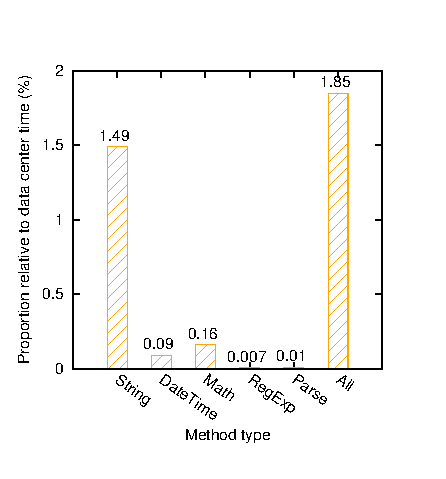
\includegraphics{graphs/methodTypes}
\caption{Relevance of .NET framework method types (cosmos11)}
\label{fig:methodTypes}
\end{figure}

Figure~\ref{fig:methodTypes} illustrates the most important method types for data center cosmos11. The results are comparable for other data centers. \emph{String} methods dominate and they count as the only source of non-native code in  1.49\% of the time spent in potentially optimizable vertices. Other method types are significantly less relevant, but when combined they influence 1.85\% of the data center time. These studies show the potential for improving data center performance by providing more intrinsics and thus enabling more C++ translation.






